\documentclass{techbrief}

\usepackage{tikz, pgfplots}
\usetikzlibrary{positioning,calc,arrows,arrows.meta, shapes, decorations.markings}
\usetikzlibrary{decorations.pathreplacing}

\title{Non-linear representations in quantum mechanics}
\author{Gabriele Carcassi}
\category{Quantum mechanics}
\tags{Hilbert space, Projective space, collinear maps}

\begin{document}
	
\maketitle
	
\begin{abstract}
	The linear representation of quantum theory in terms of vector spaces is not a physical requirement but a convenient mathematical representation. We show this by providing a non-linear map that preserves the Born rule, and therefore all the physics.
\end{abstract}

\section{Introduction}

It is often stated that the linearity of quantum mechanics is a critical part of the theory. That is, that physical concepts, like observables and time evolution, must be represented with linear structures. Here we show that this linearity is not actually a physical requirement, and one can, in fact, represent quantum theory with non-linear objects. This means that linearity is more a convenient choice of representation than a physically meaningful requirement.

\section{Mathematical prerequisites}

First, we construct a non-linear map on a two-dimensional complex Hilbert space that preserves the projective space and its geometry.

\begin{prop}\label{nonlinearMap}
	Let $\mathcal{H}$ be a two-dimensional complex Hilbert space. Let $v, w \in \mathcal{H}$ be two orthonormal vectors. Let $m : \mathcal{H} \to \mathcal{H}$ be the map defined by $m(0) = 0$ and, on non-zero vectors, by
	\begin{equation}
		\begin{aligned}
			m(a v + b w) = e^{\imath \theta \frac{|a|^2}{|a|^2+|b|^2}} ( a v + b w),
		\end{aligned}
	\end{equation}
	with $\theta \in (0, 2\pi)$. Then $m$ is a bijective non-linear map that preserves rays and the Fubini--Study geodesic distance. That is, for all $x,y \in \mathcal{H} \setminus \{0\}$
	$$
	m(v+w)\neq m(v)+m(w)
	\qquad
	[m(x)]=[x],
	\qquad
	\arccos \frac{|\<m(x),m(y)\>|}{\|m(x)\|\|m(y)\|}=\arccos \frac{|\<x,y\>|}{\|x\|\|y\|}.
	$$
	The inverse is given by the same formula with $\theta$ replaced by $- \theta$.
\end{prop}

\begin{proof}
	First, let us show that the map preserves rays. For $x=av+bw\neq0$, write
	\begin{equation*}
		r(x)=\frac{|a|^2}{|a|^2+|b|^2},
		\qquad
		m(x)=e^{\imath\theta r(x)}x.
	\end{equation*}
	Since $m(x)$ differs from $x$ only by a phase factor, they belong to the same ray. Therefore $[m(x)]=[x]$.
	
	The Fubini--Study geodesic distance is also preserved. For non-zero $x,y\in\mathcal{H}$,
	\begin{equation*}
		\begin{aligned}
			\langle m(x),m(y)\rangle
			&=e^{-\imath\theta r(x)}e^{\imath\theta r(y)}
			\langle x,y\rangle
			=e^{\imath\theta(r(y)-r(x))}\langle x,y\rangle,\\
			\|m(x)\|
			&=|e^{\imath\theta r(x)}|\,\|x\|=\|x\|.
		\end{aligned}
	\end{equation*}
	The same norm identity holds for $y$. Therefore,
	\begin{equation*}
		\begin{aligned}
			\frac{|\langle m(x),m(y)\rangle|}
			{\|m(x)\|\|m(y)\|}
			&=\frac{|e^{\imath\theta(r(y)-r(x))}|\,
				|\langle x,y\rangle|}
			{\|x\|\|y\|} =\frac{|\langle x,y\rangle|}{\|x\|\|y\|}.
		\end{aligned}
	\end{equation*}
	Taking the arccosine of both sides gives the equality of distances.
	
	To establish bijectivity, note that for every $t\in\mathbb{R}$,
	\begin{equation*}
		\begin{aligned}
			r(e^{\imath t}x)
			&=\frac{|e^{\imath t}a|^2}
			{|e^{\imath t}a|^2+|e^{\imath t}b|^2} =\frac{|e^{\imath t}|^2|a|^2}
			{|e^{\imath t}|^2(|a|^2+|b|^2)}
			=r(x).
		\end{aligned}
	\end{equation*}
	Define $n(0)=0$ and $n(x)=e^{-\imath\theta r(x)}x$ for $x\neq0$. Thus $r(n(x))=r(m(x))=r(x)$, and
	\begin{equation*}
		\begin{aligned}
			m(n(x))
			&=e^{\imath\theta r(n(x))}
			e^{-\imath\theta r(x)}x
			=e^{\imath\theta r(x)}
			e^{-\imath\theta r(x)}x=x,\\
			n(m(x))
			&=e^{-\imath\theta r(m(x))}
			e^{\imath\theta r(x)}x
			=e^{-\imath\theta r(x)}
			e^{\imath\theta r(x)}x=x.
		\end{aligned}
	\end{equation*}
	Both identities also hold at zero. Therefore $m$ is bijective, with inverse $n$, given by replacing $\theta$ with $-\theta$.
	
	Finally,
	\begin{equation*}
		\begin{aligned}
			m(v)&=e^{\imath\theta}v,
			& m(w)&=w,\\
			m(v+w)&=e^{\imath\theta/2}v+e^{\imath\theta/2}w,
			& m(v)+m(w)&=e^{\imath\theta}v+w.
		\end{aligned}
	\end{equation*}
	Since $0<\theta/2<\pi$, we have $e^{\imath\theta/2}\neq1$. The coefficients of $w$ therefore differ, so linear independence gives $m(v+w)\neq m(v)+m(w)$. Hence $m$ is non-linear.
\end{proof}

\begin{coro}\label{nonlinearOperators}
	Let $m$ be the map in the preceding proposition. A linear operator
	$A:\mathcal{H}\to\mathcal{H}$ transported through $m$,
	\begin{equation*}
		\widetilde A=m\circ A\circ m^{-1},
	\end{equation*}
	need not be linear with respect to the ordinary vector-space
	structure on $\mathcal{H}$, even when $A$ is both self-adjoint
	and unitary.
\end{coro}

\begin{proof}
	Define $A(av+bw)=bv+aw$. In the orthonormal basis $(v,w)$,
	\begin{equation*}
		A=\begin{pmatrix}0&1\\1&0\end{pmatrix},
		\qquad
		A^*=A,
		\qquad
		A^*A=A^2=I.
	\end{equation*}
	Thus $A$ is linear, self-adjoint and unitary. Using the inverse
	formula for $m$, we obtain
	\begin{equation*}
		\begin{aligned}
			\widetilde A(v)
			&=m\!\left(A(e^{-\imath\theta}v)\right)
			=m(e^{-\imath\theta}w)
			=e^{-\imath\theta}w,\\
			\widetilde A(w)
			&=m(A(w))=m(v)=e^{\imath\theta}v,\\
			\widetilde A(v+w)
			&=m\!\left(A(e^{-\imath\theta/2}(v+w))\right)\\
			&=m(e^{-\imath\theta/2}(v+w))\\
			&=e^{\imath\theta/2}e^{-\imath\theta/2}(v+w)
			=v+w.
		\end{aligned}
	\end{equation*}
	However,
	\begin{equation*}
		\widetilde A(v)+\widetilde A(w)
		=e^{\imath\theta}v+e^{-\imath\theta}w.
	\end{equation*}
	Since $0<\theta<2\pi$, we have $e^{\imath\theta}\neq1$.
	The coefficients of $v$ therefore differ, so linear independence gives
	$\widetilde A(v+w)\neq\widetilde A(v)+\widetilde A(w)$.
	Hence $\widetilde A$ is non-linear.
\end{proof}

\section{Conditions}

We can sum up the definitions of a state space in quantum mechanics with the following condition.

\begin{condition}[Quantum states]{QST:H}
	The state space of a quantum system is represented by the projective space $\mathcal{P}(\mathcal{H})$ of a separable complex Hilbert space $\mathcal{H}$. The ensemble space is represented by the density operators $\mathcal{D}(\mathcal{H})$. The conditional probability is given by the Born rule $p(\psi|\phi) = \frac{\< \phi | \psi \>\< \psi | \phi \>}{\< \psi | \psi \>\< \phi | \phi \>}$. The entropy is given by the von Neumann entropy $S(\rho) = -\tr(\rho \log \rho)$.
\end{condition}

The following condition requires other physical objects to be represented by linear structures and operations on $\mathcal{H}$.
\begin{condition}[Linear vector space representation]{QMLIN}
	Whenever quantum states are represented as rays of a Hilbert space, superpositions, observables, and evolution must be represented using the ordinary linear structure of that Hilbert space. That is, quantum superpositions are represented by vector addition, observables by self-adjoint operators and system evolution by unitary operators.
\end{condition}

\section{Theorem}

\begin{thrm}[Linearity is a choice]
	Condition \ref{QMLIN} is false.
\end{thrm}

\begin{figure}[h]
	\centering
	
	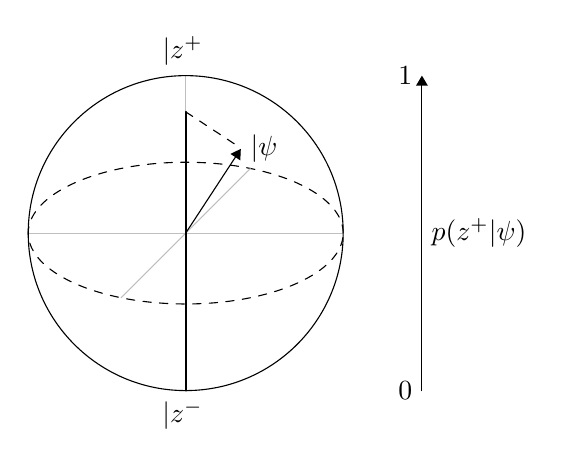
\begin{tikzpicture}[scale = 1.0, line cap=round, line join=round, >=Triangle]
		% equator
		\draw [rotate around={0.:(0.,0.)},dash pattern=on 3pt off 3pt] (0,0) ellipse (2cm and 0.9cm);
		% axis
		\draw [lightgray] (0,-2) -- (0,2);
		\draw [lightgray] (0.82,0.82) -- (-0.82,-0.82);
		\draw [lightgray] (-2,0) -- (2,0);
		% main circle
		\draw(0,0) circle (2cm);
		\draw [->] (0,0) -- (0.70,1.07);
		\draw [dashed] (0,1.54) -- (0.7,1.08);
		\draw [thick] (0,-2) -- (0,1.54);
		% symbols
		\draw (0.70,1.07) node[right] {$|\psi\>$};
		\draw (0,2) node[above] {$|z^+\>$};
		\draw (0,-2) node[below] {$|z^-\>$};
		\draw [->] (3,-2) -- node[right] {$p(z^+|\psi)$} (3,+2);
		\draw (3,-2) node[left] {$0$};
		\draw (3,2) node[left] {$1$};
		
		%\draw (0.4,1.65) node[anchor=north west] {$|\psi\>$};
		% decoration
		\scriptsize
		%\draw [fill] (0,0) circle (1.5pt);
		%\draw [fill] (0.7,1.1) circle (0.5pt);
	\end{tikzpicture} 
	\caption{\label{figNonLinearMap} Probability is vertical height on the Bloch sphere. The map $m$ introduces a phase shift on the vectors that is proportional to the vertical height, while leaving each pure-state point unchanged on the Bloch sphere.}
\end{figure}

\begin{proof}
	To show that \ref{QMLIN} is false, it suffices to provide a valid representation for a single quantum system that does not obey \ref{QMLIN}. Consider $m$ as defined by \ref{nonlinearMap} with $v = |z^+\>$ and $w = | z^- \>$. Note that $\frac{|a|^2}{|a|^2+|b|^2} = p(z^+|\psi)$ with $|\psi\rangle=a|z^+\rangle+b|z^-\rangle$. This means that the phase shift introduced by the map is proportional to the probability of measuring $z^+$.

	Since $m$ is a bijection, physical representatives on $\mathcal{H}$ transported through $m$ will be physical representatives on $m(\mathcal{H})$. Since $m$ preserves rays, the state representation is unchanged. Similarly, density operators will be left unchanged together with their entropy. The Born rule is left unchanged as it is the cosine square of the Fubini--Study distance. Therefore, \ref{QST:H} remains valid on $m(\mathcal{H})$.
	
	However, by \ref{nonlinearMap} and \ref{nonlinearOperators}, linear combinations and linear operators do not correspond, in general, to transported linear combinations and linear operators. Therefore, quantum superposition in one representation will not, in general, map to the same linear combinations. Similarly, observables will not be, in general, represented by self-adjoint operators and time evolution will not be, in general, represented by unitary maps.
	
	We therefore have a representation where \ref{QST:H} holds but superpositions, observables and time evolution are not represented by the ordinary linear structures. Therefore \ref{QMLIN} is false.
\end{proof}	

\section{Conclusion}

We have shown that non-linear maps that do not conserve the inner product but preserve the Born rule, and thus all the physics, exist and therefore the linear representation amounts to a choice of representation. We should also note that alternative representations exist that are not even tied to vector spaces: the Madelung equations (also known as the equations of quantum hydrodynamics) provide such a representation.

\end{document}
